\documentclass[12pt,a4paper]{article}
\usepackage{hyperref}
\usepackage{graphicx}
\graphicspath{{Documentation/figures/}}
\usepackage{listings}
\usepackage{xcolor}
\usepackage{amsmath}
\usepackage[utf8]{inputenc}
\usepackage{amsthm}
\usepackage{float}
\usepackage{algorithm}
\usepackage{algpseudocode}
\usepackage{dirtree}
\usepackage[a4paper, top=1in, bottom=0.8in, left=1in, right=1in]{geometry}

\newtheorem{definition}{Definition}
\definecolor{codegreen}{rgb}{0,0.6,0}
\definecolor{codegray}{rgb}{0.5,0.5,0.5}
\definecolor{codepurple}{rgb}{0.58,0,0.82}
\definecolor{backcolour}{rgb}{0.95,0.95,0.92}

\lstdefinestyle{mystyle}{
    backgroundcolor=\color{backcolour},
    commentstyle=\color{codegreen},
    keywordstyle=\color{magenta},
    numberstyle=\tiny\color{codegray},
    stringstyle=\color{codepurple},
    basicstyle=\ttfamily\footnotesize,
    breakatwhitespace=false,
    breaklines=true,
    captionpos=b,
    keepspaces=true,
    numbers=left,
    numbersep=5pt,
    showspaces=false,
    showstringspaces=false,
    showtabs=false,
    tabsize=2
}

\lstset{style=mystyle}

\title{\bfseries InsightDash \\ \large Interactive KPI Intelligence Platform}
\author{Owen}
\date{\today}

\begin{document}

\begin{titlepage}
    \centering
    \vspace*{\fill}
    {\bfseries\Huge InsightDash \par}
    \vspace{0.5cm}
    {\Large KPI Intelligence Platform \par}
    \vspace{1.5cm}
    {\large Owen \par}
    \vspace{0.5cm}
    {\large \today \par}
    \vspace*{\fill}
\end{titlepage}

\tableofcontents{}
\newpage

\section{Introduction}

\begin{flushleft}
InsightDash is an analytics dashboard that pulls data from SQL Server and turns it into interactive charts. It features AI-powered summaries to explain key trends directly on the screen, providing a ready-to-use command centre for business leaders.
\end{flushleft}

\section{System Architecture}

The runtime is orchestrated from the Dash entry point (\texttt{app.py}) and flows as follows:

\begin{enumerate}
    \item Configure structured logging and read environment-driven settings (database, LLM, feature switches).
    \item Fetch per-tab datasets by executing templated SQL through SQLAlchemy engines.
    \item Normalise and remap query outputs to match the figure contracts expected by each tab.
    \item Initialise Dash layouts, set up shared colour palettes, and register interactive callbacks within \texttt{app.py}.
    \item Serve interactive charts that support cross-filtering, drill-down, and multi-select synchronisation.
    \item Use the Gemini LLM to produce quantified narratives and insights for any graph on demand.
    \item Persist usage logs and optional insight markdown while keeping the UI responsive.
\end{enumerate}

\newpage
\subsection{Project Structure}

\dirtree{%
.1 InsightDash \DTcomment{Root for the interactive analytics app}.
.2 app.py \DTcomment{Dash bootstrapper and callback wiring}.
.2 app\_tabs.
.3 tab1 \DTcomment{Outlet performance view}.
.4 figures.py \DTcomment{Plotly graph builders}.
.4 layout.py \DTcomment{Tab layout components}.
.3 tab2 \DTcomment{Dynamic scatter plot view}.
.4 figures.py.
.4 layout.py.
.3 tab3 \DTcomment{Trend and ranking view}.
.4 figures.py.
.4 layout.py.
.2 assets.
.3 styles.css \DTcomment{Global styling overrides}.
.3 sidebar\_controls.css \DTcomment{Resizable panel theming}.
.2 config.
.3 settings.py \DTcomment{Environment flags and connection URIs}.
.3 logging.py. 
.2 data\_layer.
.3 base.py \DTcomment{Shared SQL execution helpers}.
.3 tab\_1.py \DTcomment{Tab-specific query orchestration}.
.3 tab\_2.py.
.3 tab\_3.py.
.2 services.
.3 llm.py \DTcomment{Gemini client abstraction}.
.3 insights.py \DTcomment{Chunked summarisation logic}.
.3 prompts.py \DTcomment{Prompt builders for Gemini}.
.2 sql\_queries \DTcomment{Templated SQL per tab}.
.2 utils.
.3 data.py \DTcomment{Deduplication and packing helpers}.
.3 colors.py \DTcomment{Palette utilities and colour maps}.
.3 dataframe.py \DTcomment{NaN handling and concatenation helpers}.
.3 df\_summary.py \DTcomment{Basic statistics for LLM payloads}.
.2 logs \DTcomment{Usage and diagnostic output}.
.2 InsightDash.pdf \DTcomment{Project documentation (this file)}.
}

\subsection{Component Diagram}

\begin{center}
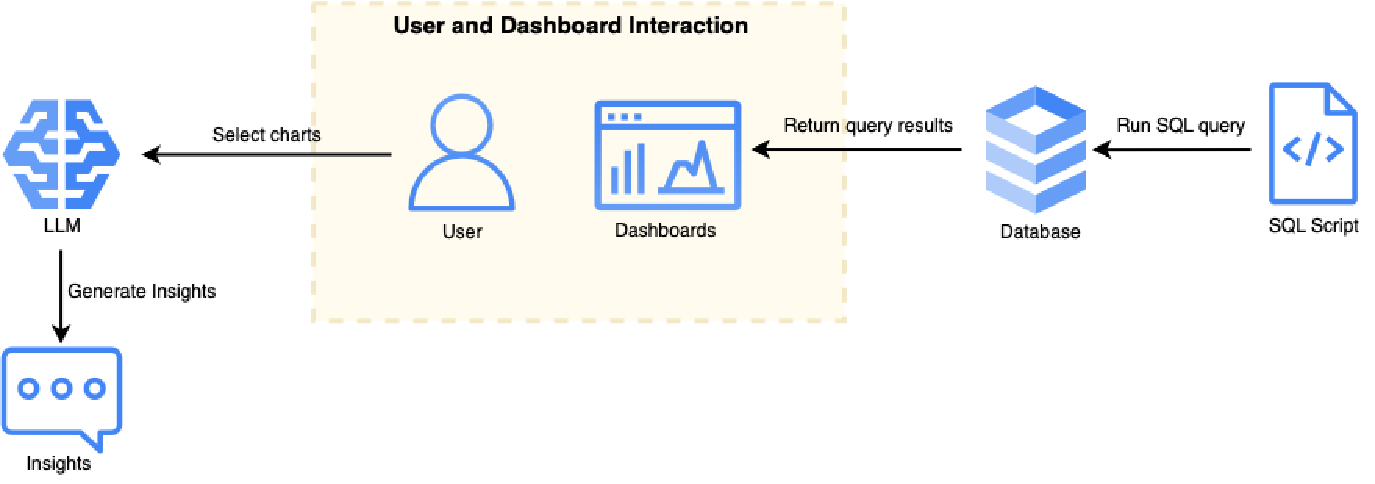
\includegraphics[width=0.95\textwidth]{figures/InsightDashMap.pdf}
\end{center}

\begin{enumerate}
\item \textbf{SQL Script}: Executes predefined queries.
\item \textbf{Database}: The data source queried to extract the necessary KPI data.
\item \textbf{Dashboards}: Visualizes the extracted data through interactive charts and graphs.
\item \textbf{Users}: Apply filters and request AI-generated insights.
\item \textbf{LLM}: Generates narrative insights based on the data from the user's selected charts.
\end{enumerate}

\section{Implementation}
\subsection{Runtime Algorithm}

The Dash application follows the control flow summarised in Algorithm~\ref{alg:runtime}. Each stage is idempotent, enabling hot-reload in development and reliable deployments.

\begin{algorithm}[H]
\caption{InsightDash Runtime Lifecycle (\texttt{app.py})}
\label{alg:runtime}
\begin{algorithmic}[1]
\Require Environment variables, SQL templates, Plotly Dash runtime
\Ensure Responsive dashboard with optional LLM summaries
\State \Call{configure\_logging}{}
\State data\_tab1 $\gets$ \Call{get\_tab1\_results}{"kpi\_april"}
\State data\_tab2 $\gets$ \Call{get\_tab2\_results}{"kpi\_april"}
\State data\_tab3 $\gets$ \Call{get\_tab3\_results}{"kpi\_april"}
\State monthly $\gets$ \Call{load\_additional\_months}{["kpi\_may", ...]}
\State app $\gets$ \Call{create\_dashboard}{data\_tab1, data\_tab2, data\_tab3, monthly}
\While{app is running}
    \State Process callback inputs and recompute filtered DataFrames
    \If{user requests insight}
        \State slices $\gets$ \Call{chunk\_dataframe}{selection}
        \State chunk\_notes $\gets$ \Call{summarize\_chart\_via\_chunks}{slices, context}
        \State markup $\gets$ \Call{synthesize\_across\_charts}{chunk\_notes}
        \State Update markdown panel with $markup$
    \EndIf
    \State Append usage metrics to \texttt{logs/usage.log}
\EndWhile
\end{algorithmic}
\end{algorithm}

\subsection{Flow Chart}

\begin{figure}[H]
    \centering
    \makebox[\textwidth][c]{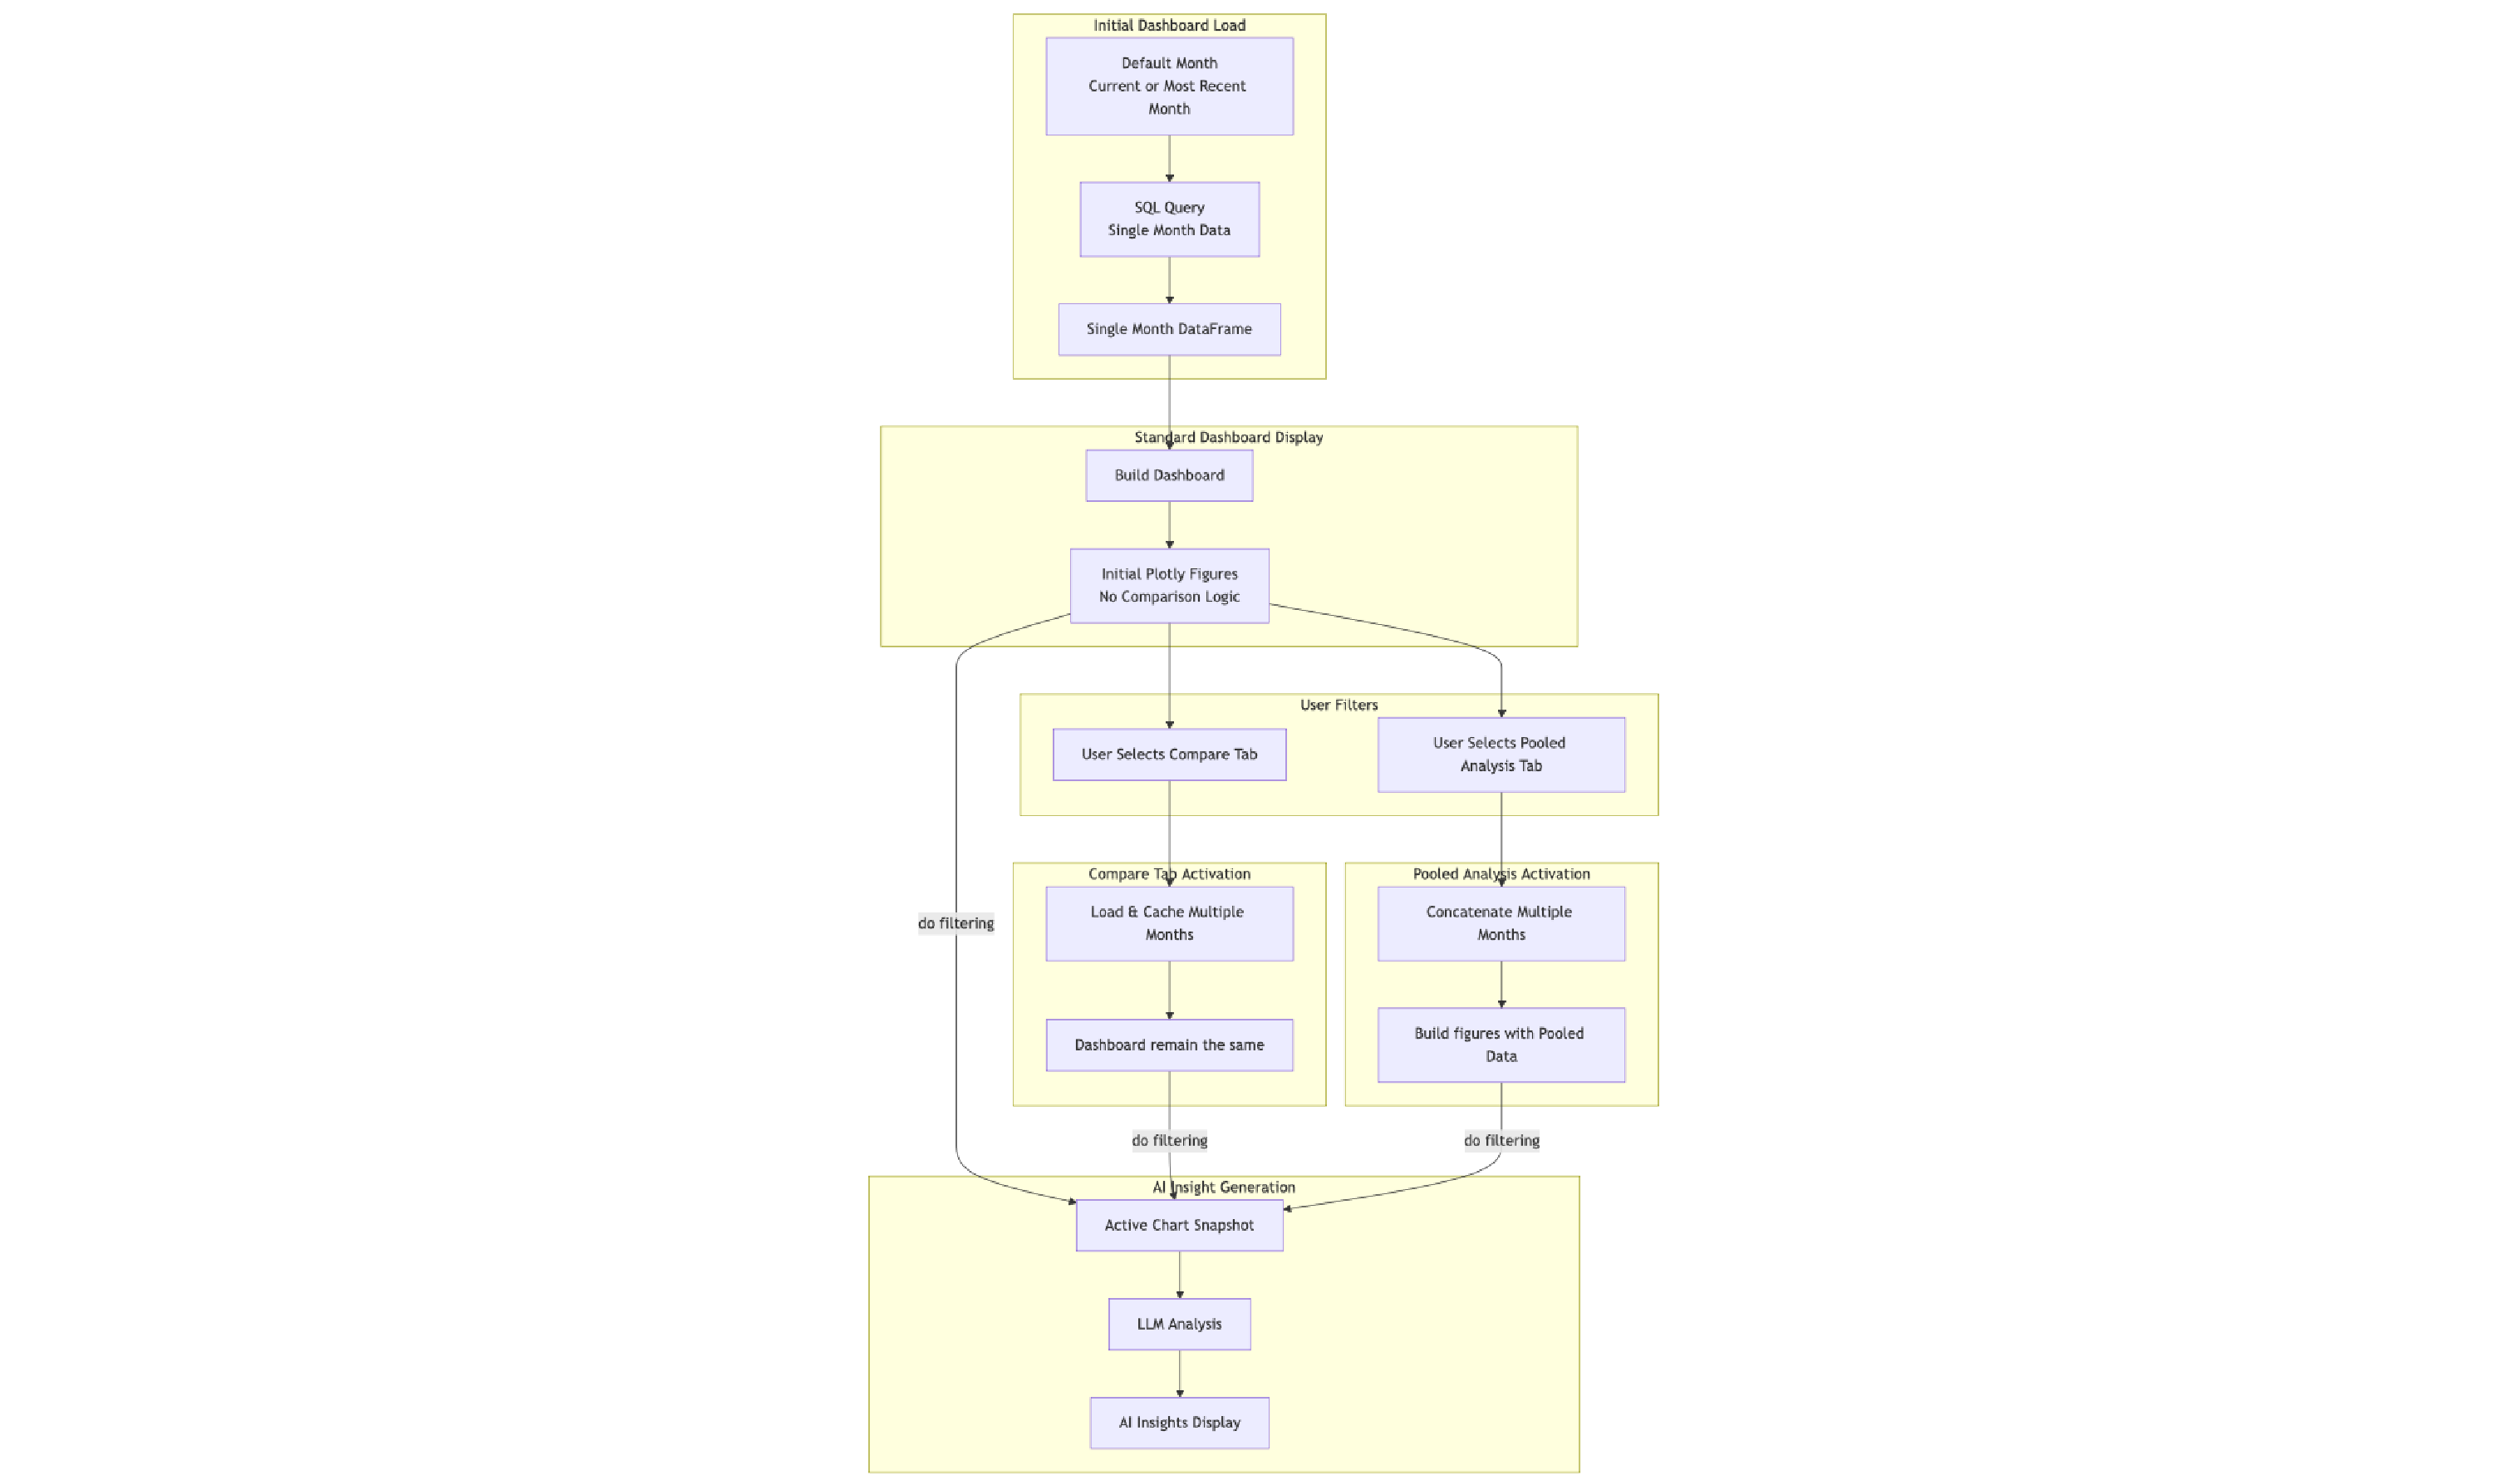
\includegraphics[width=2.5\textwidth]{figures/flowchart.pdf}}
\end{figure}

\subsection{Key Modules}

\begin{itemize}
    \item \textbf{\texttt{app.py}}: Entry point that builds the Dash instance, injects tab layouts, and defines callback wiring for filters, graph selections, and insight generation.
    \item \textbf{\texttt{data\_layer/*}}: Encapsulates SQL execution, result validation, and schema remediation so downstream charts always receive the expected columns.
    \item \textbf{\texttt{app\_tabs/*/figures.py}}: Houses Plotly figure factories and table builders, isolating complex styling logic from callbacks.
    \item \textbf{\texttt{services/insights.py}}: Implements the map-reduce summarisation pipeline, including basic statistics to generate a consistent LLM outputs.
    \item \textbf{\texttt{utils/colors.py} \& \texttt{utils/data.py}}: Provide consistent colour assignments, deduplication helpers, and DataFrame serialisation utilities shared across tabs.
    \item \textbf{\texttt{assets/*.css}}: Defines the visual identity (typography, spacing, panel controls) to keep charts and sidebars visually cohesive.
\end{itemize}

\section{Related Technologies and References}

\begin{itemize}
    \item \href{https://dash.plotly.com/}{Plotly Dash documentation} for component APIs and layout patterns.
    \item \href{https://docs.sqlalchemy.org/}{SQLAlchemy} for engine creation and query execution against SQL Server.
    \item \href{https://ai.google.dev/docs/gemini_api_overview}{Google Gemini API} for configuring the LLM insight features.
    \item \href{https://loguru.readthedocs.io/}{Loguru} for advanced logging patterns used by the project.
\end{itemize}

\section{Frequently Asked Questions}

\begin{itemize}
    \item \textbf{How do monthly KPI tables map to dashboard tabs?}\\
    Each tab module builds a SQL map using the configured month (e.g., \texttt{kpi\_april}). The keys (\texttt{q1}, \texttt{q2}, etc.) line up with figure factories that expect specific schemas.
    \item \textbf{What ensures colour consistency across tabs?}\\
    \texttt{utils.colors.color\_map\_from\_list} generates deterministic palette assignments based on sorted category lists, and the results are cached per session.
    \item \textbf{Where are usage analytics stored?}\\
    Loguru writes structured entries to \texttt{logs/usage.log}, tagging events with \texttt{usage=True} so downstream tooling can aggregate adoption metrics.
    \item \textbf{How do I add a new KPI tab?}\\
    Scaffold a new folder under \texttt{app\_tabs}, implement \texttt{layout.py} and \texttt{figures.py}, then wire new callbacks inside \texttt{app.py} (or a dedicated module) and extend \texttt{data\_layer} to supply the required SQL results.
\end{itemize}

\end{document}
